\documentclass[journal,12pt,twocolumn]{IEEEtran}

\usepackage{setspace}
\usepackage{gensymb}
\singlespacing
\usepackage[cmex10]{amsmath}

\usepackage{amsthm}

\usepackage{mathrsfs}
\usepackage{txfonts}
\usepackage{stfloats}
\usepackage{bm}
\usepackage{cite}
\usepackage{cases}
\usepackage{subfig}
\usepackage{paralist}
\usepackage{longtable}
\usepackage{multirow}

\usepackage{enumitem}
\usepackage{mathtools}
\usepackage{steinmetz}
\usepackage{tikz}
\usepackage{circuitikz}
\usepackage{verbatim}
\usepackage{tfrupee}
\usepackage[breaklinks=true]{hyperref}
\usepackage{graphicx}
\usepackage{tkz-euclide}

\usetikzlibrary{calc,math}
\usepackage{listings}
    \usepackage{color}                                            %%
    \usepackage{array}                                            %%
    \usepackage{longtable}                                        %%
    \usepackage{calc}                                             %%
    \usepackage{multirow}                                         %%
    \usepackage{hhline}                                           %%
    \usepackage{ifthen}                                           %%
    \usepackage{lscape}     
\usepackage{multicol}
\usepackage{chngcntr}


\usetikzlibrary{calc,math}
\usepackage{listings}
    \usepackage{color}                                            %%
    \usepackage{array}                                            %%
    \usepackage{longtable}                                        %%
    \usepackage{calc}                                             %%
    \usepackage{multirow}                                         %%
    \usepackage{hhline}                                           %%
    \usepackage{ifthen}                                           %%
    \usepackage{lscape}     
\usepackage{multicol}
\usepackage{chngcntr}
\newtheorem{theorem}{Theorem}[section]
\newtheorem{lemma}[theorem]{Lemma}

\DeclareMathOperator*{\Res}{Res}

\renewcommand\thesection{\arabic{section}}
\renewcommand\thesubsection{\thesection.\arabic{subsection}}
\renewcommand\thesubsubsection{\thesubsection.\arabic{subsubsection}}

\renewcommand\thesectiondis{\arabic{section}}
\renewcommand\thesubsectiondis{\thesectiondis.\arabic{subsection}}
\renewcommand\thesubsubsectiondis{\thesubsectiondis.\arabic{subsubsection}}


\hyphenation{op-tical net-works semi-conduc-tor}
\def\inputGnumericTable{}                                 %%

\lstset{
%language=C,
frame=single, 
breaklines=true,
columns=fullflexible
}
\begin{document}

\newcommand{\BEQA}{\begin{eqnarray}}
\newcommand{\EEQA}{\end{eqnarray}}
\newcommand{\define}{\stackrel{\triangle}{=}}
\newcommand{\R}{\mathbb{R}}
\bibliographystyle{IEEEtran}
\raggedbottom
\setlength{\parindent}{0pt}
\providecommand{\mbf}{\mathbf}
\providecommand{\pr}[1]{\ensuremath{\Pr\left(#1\right)}}
\providecommand{\qfunc}[1]{\ensuremath{Q\left(#1\right)}}
\providecommand{\sbrak}[1]{\ensuremath{{}\left[#1\right]}}
\providecommand{\lsbrak}[1]{\ensuremath{{}\left[#1\right.}}
\providecommand{\rsbrak}[1]{\ensuremath{{}\left.#1\right]}}
\providecommand{\brak}[1]{\ensuremath{\left(#1\right)}}
\providecommand{\lbrak}[1]{\ensuremath{\left(#1\right.}}
\providecommand{\rbrak}[1]{\ensuremath{\left.#1\right)}}
\providecommand{\cbrak}[1]{\ensuremath{\left\{#1\right\}}}
\providecommand{\lcbrak}[1]{\ensuremath{\left\{#1\right.}}
\providecommand{\rcbrak}[1]{\ensuremath{\left.#1\right\}}}
\theoremstyle{remark}
\newtheorem{rem}{Remark}
\newcommand{\sgn}{\mathop{\mathrm{sgn}}}
\providecommand{\abs}[1]{\vert#1\vert}
\providecommand{\res}[1]{\Res\displaylimits_{#1}} 
\providecommand{\norm}[1]{\lVert#1\rVert}
%\providecommand{\norm}[1]{\lVert#1\rVert}
\providecommand{\mtx}[1]{\mathbf{#1}}
\providecommand{\mean}[1]{E[ #1 ]}
\providecommand{\fourier}{\overset{\mathcal{F}}{ \rightleftharpoons}}
%\providecommand{\hilbert}{\overset{\mathcal{H}}{ \rightleftharpoons}}
\providecommand{\system}{\overset{\mathcal{H}}{ \longleftrightarrow}}
	%\newcommand{\solution}[2]{\textbf{Solution:}{#1}}
\newcommand{\solution}{\noindent \textbf{Solution: }}
\newcommand{\cosec}{\,\text{cosec}\,}
\providecommand{\dec}[2]{\ensuremath{\overset{#1}{\underset{#2}{\gtrless}}}}
\newcommand{\myvec}[1]{\ensuremath{\begin{pmatrix}#1\end{pmatrix}}}
\newcommand{\mydet}[1]{\ensuremath{\begin{vmatrix}#1\end{vmatrix}}}
\numberwithin{equation}{subsection}
\makeatletter
\@addtoreset{figure}{problem}
\makeatother
\let\StandardTheFigure\thefigure
\let\vec\mathbf
\renewcommand{\thefigure}{\theproblem}
\def\putbox#1#2#3{\makebox[0in][l]{\makebox[#1][l]{}\raisebox{\baselineskip}[0in][0in]{\raisebox{#2}[0in][0in]{#3}}}}
     \def\rightbox#1{\makebox[0in][r]{#1}}
     \def\centbox#1{\makebox[0in]{#1}}
     \def\topbox#1{\raisebox{-\baselineskip}[0in][0in]{#1}}
     \def\midbox#1{\raisebox{-0.5\baselineskip}[0in][0in]{#1}}
\vspace{3cm}
\title{AI1103-Assignment 4}
\author{Name: Avula Mohana Durga Dinesh Reddy , Roll Number: CS20BTECH11005}
\maketitle
\newpage
\bigskip
\renewcommand{\thefigure}{\theenumi}
\renewcommand{\thetable}{\theenumi}
Download all python codes from 
\begin{lstlisting}
https://github.com/DineshAvulaMohanaDurga/AI1103/blob/main/assignment_4_new/codes/ai1103_assignment4 new.py
\end{lstlisting}
%
and latex codes from 
%
\begin{lstlisting}
https://github.com/DineshAvulaMohanaDurga/AI1103/blob/main/assignment_4_new/main.tex
\end{lstlisting}
\section{Question}
\brak{\text{CSIR-UGC-NET June 2015 Q 110}}Suppose X has density $f\brak{\frac{x}{\theta}}=\frac{1}{\theta} e^{-x/\theta},x>0$ where $\theta > 0$ is unknown.Define Y as follows:\\
Y=k if $k \leq X < k+1$, k=0,1,2 $\cdots$\\
Then the distribution of Y is :
\begin{enumerate}
\item Normal 
\item Binomial 
\item Poisson 
\item Geometric
\end{enumerate}
\section{Answer}
\begin{lemma}
If the pdf of X is in the form of 
\begin{align}
p\brak{X=x}&=\brak{1-p}^{x} p, \text{ where } \brak{x=0,1,2,\cdots}
\end{align} 
Then the distribution is said to be in the form of geometric distribution. 
\end{lemma}
\begin{lemma}
pdf of X is 
\begin{align}
\pr{X}&=\frac{1}{\theta} e^{-\frac{x}{\theta}}
\end{align}
\end{lemma}
\begin{proof}
Given pdf of X is 
\begin{align}
f\brak{x | \theta}&=\frac{1}{\theta} e^{-x/\theta},x>0,\text{where } \theta >0 \text{ is unknown}\\
f\brak{x}&=\frac{1}{\theta}e^{-\frac{x}{\theta}} \text{since x and }\theta \text{ are independent} 
\end{align}
Hence lemma 2.2 is proved.
\end{proof}
\begin{lemma}
pdf of Y is 
\begin{align}
p\brak{Y=k}&=e^{-\frac{k}{\theta}} \brak{1-e^{-\frac{k}{\theta}}}
\end{align}
and is in the form of geometric distribution.
\end{lemma}
\begin{proof}
Also given that Y=k if $k \leq X <k+1$ k=0,1,2,$\cdots$
\begin{align}
p\brak{Y=k}&=\int_k^{k+1} p\brak{X=x} dx\\
&=\int_k^{k+1} \frac{1}{\theta} e^{-\frac{x}{\theta}} dx \nonumber \\
&=e^{-\frac{k}{\theta}} \brak{1-e^{-\frac{k}{\theta}}} \label{PDF of Y}
\end{align}
Hence using lemma 2.1  and (\ref{pdf of Y}) lemma 2.3 is proved.
\end{proof}`
\begin{figure}[ht]
    \centering
    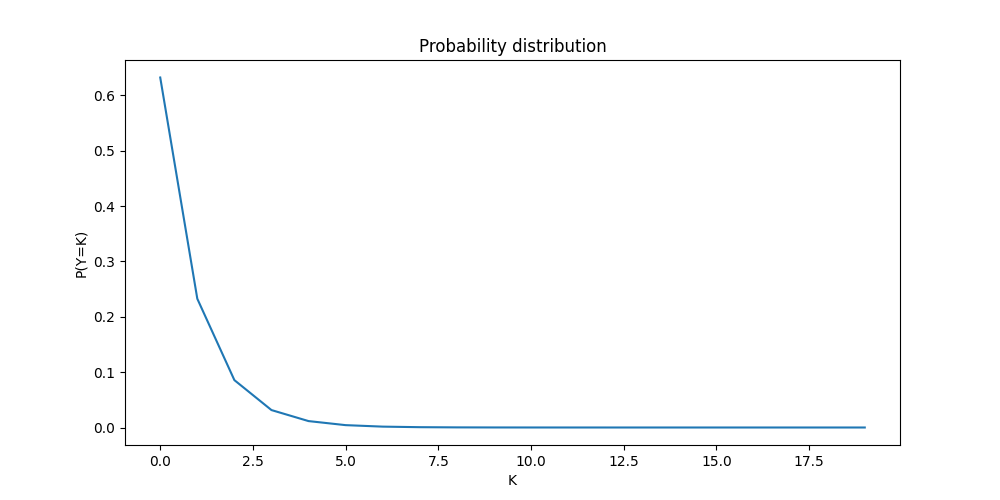
\includegraphics[width=0.5\textwidth]{Figure_1.png}
    \caption{Probability distribution of Y}
    \label{fig:my_label}
\end{figure}
\end{document}